\documentclass[12pt]{article}
\usepackage[utf8x]{inputenc}
\usepackage[italian,english]{babel}
\usepackage{url,graphicx,tabularx,array,geometry}
\usepackage{amsmath}
\setlength{\parskip}{1ex} 
\setlength{\parindent}{0pt} 
\usepackage{listings}
\usepackage{tikz}
%\renewcommand{\title}[1]{\textbf{#1}\\}
\renewcommand{\line}{\begin{tabularx}{\textwidth}{X>{\raggedleft}X}\hline\\\end{tabularx}\\[-0.5cm]}
\newcommand{\leftright}[2]{\begin{tabularx}{\textwidth}{X>{\raggedleft}X}#1%
& #2\\\end{tabularx}\\[-0.5cm]}

\lstset{basicstyle=\small\ttfamily,
keywordstyle=\color{black}\bfseries,
commentstyle=\color{darkgray},
stringstyle=\color{black},
showstringspaces=true,numbers=left}

\begin{document}

\title{From MASON to D-MASON, a simple example: Particles}
\author{\url{http://www.isislab.it/projects/dmason}}
\maketitle
%\leftright{}{ISISLab}
\leftright{}{}
\leftright{}{}

\section{Introduction}
In this short document we provide a step-by-step guide to ``parallelize'' the Particle example from MASON by using D-MASON.
\begin{figure}[ht]
	\centering
		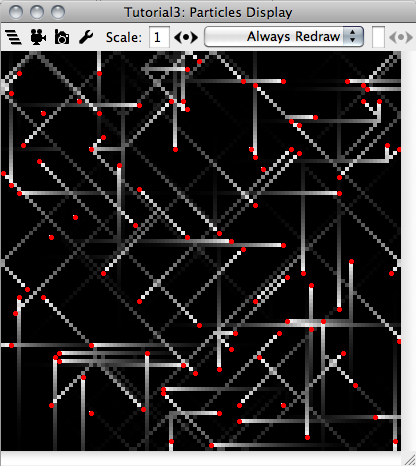
\includegraphics[width=0.5\textwidth, bb=0 0 470 520]{particles.png}	
		\caption{GUIState for \textit{Particle} simulation}
	\label{fig:p01}
\end{figure}
\section{Structure}
The starting point is the package \textbf{Particles} is composed by three classes, as it can be found in the original MASON distribution:

\begin{itemize}
	\item \textbf{Particle:} it implements the agent that will be simulated by the application.
	\item \textbf{Particles:} it represents the simulation environment: it allows to run the simulation from the command line without using a GUI.
	\item \textbf{ParticlesWithUI:} it allows to run simulations with a GUI, as depicted in the Figure \ref{fig:p01}.
\end{itemize}

Similarly, in D-MASON, there will be the package \textbf{DParticles} containing the following classes:
\begin{itemize}
	\item \textbf{RemoteParticle:} it is an abstract class, implementing \textit{RemoteAgent} and containing the remote ID of the agent in the field and its position. 
	\item \textbf{DParticle:} it extends \textit{RemoteParticle} and implements the \textit{distributed} agent that will be simulated by the application.
	\item \textbf{DParticles:} it represents the \textit{distributed} simulation environment: it allows to run the simulation from the command line without using a GUI.
	\item \textbf{DParticlesWithUI:} it allows to run simulations with a GUI that is aware of the \textit{distributed} environment.
\end{itemize}

\subsection{From Particle to DParticle}
The original \textbf{Particle} has to implement the \textit{Steppable} interface and, in particular, the method \textit{step()}, containing the agent logic. In the same way \textit{RemoteParticle} is an abstract class that has to implement \textit{RemoteAgent}, that is the D-MASON interface containing the necessary logic for the distributed agent. Finally \textit{DParticle} extends \textit{RemoteParticle} and implements the logic of the agent.

\textit{RemoteAgent} is parameterized with an \textit{Int2D} object-type because, in this simulation, the field has this specific type to indicate locations, and allows programmers to set, for each agent, an unique identifier and a field position.
A \textit{Particle} simply contains two integer parameters, \textit{xdir} and \textit{ydir}, for setting the initial direction that the particle will move along.

\lstset{language=Java,caption={Class Particle},label=particle1}
\begin{lstlisting}
...
  public Particle(int xdir, int ydir) {
   public boolean randomize = false;
   this.xdir = xdir;
   this.ydir = ydir;
  }
...
\end{lstlisting}
\medskip

\textit{DParticle} has two constructors: the first is empty and it has been introduced for a future implementation of the method \textit{clone()}, and the second one has as parameter a subclass of the abstract class \textit{DistributedState}.

\lstset{language=Java,caption={Class DParticle},label=dparticle1}
\begin{lstlisting}
public class DParticle extends RemoteParticle<Int2D>
{
   public int xdir;  // -1, 0, or 1
   public int ydir;  // -1, 0, or 1

   public DParticle(){ }
   
   public DParticle(DistributedState state)
   {
     super(state);
   }
\end{lstlisting}

In order to distribute a MASON simulation it is necessary to change some parts of the agent logic. In the original MASON version each particle, on each step, performs a collision avoidance routine by checking whether the location it is moving to is already occupied by another particle or not. 

\lstset{language=Java,caption={Class Particle},label=particle2}
\begin{lstlisting}
   ...
  public void step(SimState state) {
   ...
   if (randomize) {
    xdir = tut.random.nextInt(3) - 1;
    ydir = tut.random.nextInt(3) - 1;
	  randomize = false;
   }
   ...
   // set my new location
   Int2D newloc = new Int2D(newx,newy);
   tut.particles.setObjectLocation(this,newloc);
   
   // randomize everyone at that location if need be
   Bag p = tut.particles.getObjectsAtLocation(newloc);
   if (p.numObjs > 1) {
   for(int x=0;x<p.numObjs;x++)
       ((Particle)(p.objs[x])).randomize = true;
   }
  }
}
\end{lstlisting}

The distributed version is slightly different because it first check if the new location is occupied and, in this case, it randomizes its direction and move to the new location by using the method \textit{setDistributedObjectLocation}.

%In a distributed environment different particles cannot do this check in different steps, as in the original version, but they first check for collision, using the same MASON method, then they set the new field location, using \textit{setDistributedObjectLocation}. 

\lstset{language=Java,caption={Class DParticle},label=dparticle2}
\begin{lstlisting}
public void step(SimState state)
{
 DParticles tut = (DParticles)state;
 Int2D location = tut.particles.getObjectLocation(this);
 Bag p = tut.particles.getObjectsAtLocation(location);
 tut.trails.setDistributedObjectLocation(1.0, location,state);
 if (p.numObjs > 1)
 {
   xdir = tut.random.nextInt(3) - 1; 
   ydir = tut.random.nextInt(3) - 1;
 }
 int newx = location.x + xdir;
 int newy = location.y + ydir;
 if (newx < 0) { newx++; xdir = -xdir; } 
 else if (newx >= tut.trails.getWidth()) {newx--; xdir = -xdir; }
 if (newy < 0) { newy++ ; ydir = -ydir; }
 else if (newy >= tut.trails.getHeight()) {newy--; ydir = -ydir; }
 Int2D newloc = new Int2D(newx,newy);
 tut.particles.setDistributedObjectLocation(newloc, this, state);
 }
}
\end{lstlisting}


\subsection{From Particles to DParticles}
\textit{Particles} extends the \textit{SimState} class  while \textit{DParticles} extends \textit{DistributedState}, parameterized with \textit{Int2D} object-type.

DParticles contains three other variables indicating, respectively, width and height of the field and the way of partitioning the field (that can be one or two dimensional, as shown in Figure \ref{fig:dp01}). \textit{Particles} has just one constructor that has as parameter the random generator seed while \textit{DParticles} constructor has as input an objects array, containing several parameters specific for the distributed simulation (e.g. network address, port, etc \ldots). 

In \textit{Particles} there are two fields, the first containing the agents, the second one containing the trails. The creation of the fields and the placement of the agents in them are carried out by a simple loop that instantiates new particles with a random position and direction and place them in the proper field. 

In order to add particles to the schedule, it is possible to use \textit{scheduleRepeating()}, that allows to schedule agents repeatedly, and to add particles to the field there is \textit{setObjectLocation()}. In \textit{DParticles} there is the method \textit{createDSparseGrid2D} of the class \textit{DSparseGrid2DFactory} for creating a new distributed field. Note that it is necessary to use a factory to choose the kind of field partition. The agent initial position is computed by the method \textit{setAvailableRandomLocation()} and to add particles in the schedule it is necessary to use the method \textit{scheduleOnce()}, because in the next step a certain agent could not stay in the same part of the field, so using \textit{scheduleRepeating()} will not delete the particle from the schedule. Finally there are other three new methods: a \textit{getter} method for returning the subclass of the \textit{DistributedState}, a method for adding an agent with a given position in the field, a method for attaching a portrayal to an agent.

\lstset{language=Java,caption={Class Particles},label=particles}
\begin{lstlisting}
public class Particles extends SimState  {
  public DoubleGrid2D trails;
  public SparseGrid2D particles;
  ...
  public Particles(long seed) {
      super(seed);
  }
  
  public void start() {
   ...
   for(int i=0 ; i<numParticles ; i++) {
     p = new Particle(random.nextInt(3) - 1, random.nextInt(3) - 1);  // random direction
     schedule.scheduleRepeating(p);
     ...
     particles.setObjectLocation(p,new Int2D(x,y));  // random location
   }
  }
  
  public static void main(String[] args) {
    doLoop(Particles.class, args);
    System.exit(0);
  }
}
\end{lstlisting}
\medskip
\lstset{language=Java,caption={Class DParticles},label=dparticles}
\begin{lstlisting}
public class DParticles extends DistributedState<Int2D> {
private static boolean isToroidal=false;
public DSparseGrid2D particles;
public DDoubleGrid2D trails;
public int gridWidth ;
public int gridHeight ;
public int MODE;

public DParticles(Object[] params)
{
 super((Integer)params[2],(Integer)params[3],(Integer)params[4],
 (Integer)params[7], (Integer)params[8], (String)params[0],
 (String)params[1],(Integer)params[9], isToroidal,
 new DistributedMultiSchedule<Int2D>());
 ip = params[0]+"";
 port = params[1]+"";
 this.MODE=(Integer)params[9];
 gridWidth=(Integer)params[5];
 gridHeight=(Integer)params[6];
}

public void start()
{
 super.start();
 try
{
 trails = DDoubleGrid2DFactory.createDDoubleGrid2D(gridWidth,
  gridHeight, this, super.MAX_DISTANCE, TYPE.pos_i,
  TYPE.pos_j, super.NUMPEERS, MODE,0, false, "trails");

 particles = DSparseGrid2DFactory.createDSparseGrid2d(gridWidth,
  gridHeight, this, 
  super.MAX_DISTANCE, TYPE.pos_i,
  TYPE.pos_j,super.NUMPEERS,MODE, "particles");

 init_connection();
}catch (DMasonException e) { e.printStackTrace();}
 DParticle p=new DParticle(this);
 while(particles.size() != super.NUMAGENTS)
{
 particles.setAvailableRandomLocation(p);
 p.xdir = random.nextInt(3)-1;
 p.ydir = random.nextInt(3)-1;
 if(particles.setDistributedObjectLocationForPeer(new Int2D
   (p.pos.getX(),p.pos.getY()), p, this))
 {
 schedule.scheduleOnce(schedule.getTime()+1.0,p);
 if(particles.size() != super.NUMAGENTS)
 p=new DParticle(this);
 }
}
 Steppable decreaser = new Steppable()
{
 public void step(SimState state)
{
 trails.multiply(0.9);
}
 static final long serialVersionUID = 6330208160095250478L;
};
 schedule.scheduleRepeating(Schedule.EPOCH,2,decreaser,1);
try
{
 getTrigger().publishToTriggerTopic("Simulation cell "+particles.cellType+" ready...");
 } catch (Exception e) {
 e.printStackTrace();
 }
}

public static void main(String[] args)
{
 doLoop(DParticles.class, args);
 System.exit(0);
}
static final long serialVersionUID = 9115981605874680023L;

public DistributedField getField()
{
 return particles;
}

public SimState getState()
{
 return this;
}

public void addToField(RemoteAgent<Int2D> rm,Int2D loc)
{
 particles.setObjectLocation(rm, loc);
}

public boolean setPortrayalForObject(Object o)
 {
 return false;
 }
}

\end{lstlisting}

\subsection{From ParticlesWithUI to DParticlesWithUI}
\begin{figure}
\centering
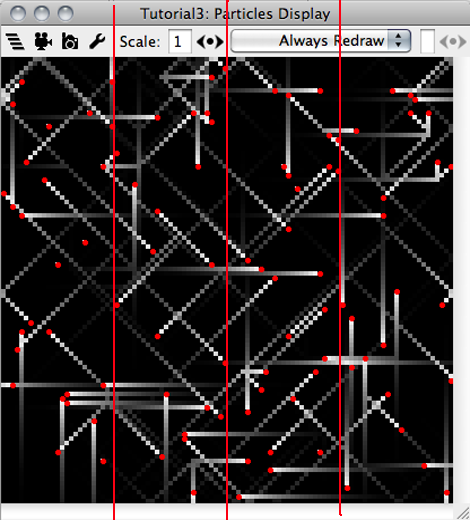
\includegraphics[width=0.4\textwidth,bb=0 0 470 520]{particles-h.png} 
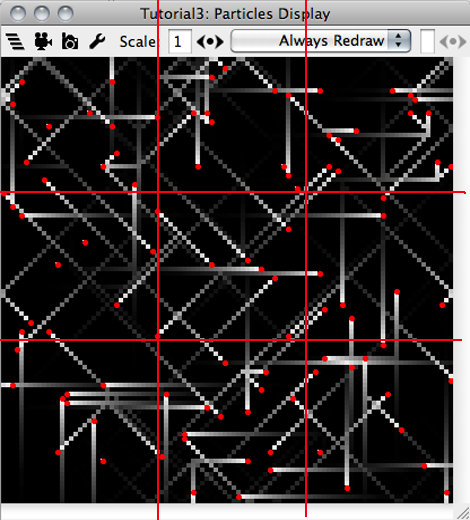
\includegraphics[width=0.4\textwidth,bb=0 0 470 520]{particles-m.png}
\caption{Respectively \textit{HORIZONTAL} and \textit{SQUARE} partition mode.}
\label{fig:dp01}
\end{figure}
There are few differences between origianl \textit{ParticlesWithUI} and the its distributed version, \textit{DParticlesWithUI}. They both extend the class \textit{GUIState}, responsible of instantiating all graphics elements; \textit{DParticlesWithUI} has a constructor for passing to \textit{DParticles} the objects array and it has to store in a \textit{String} the \textit{region} identifier, in order to show which region it is simulating (e.g. \textit{0-0} means the upper-left part of the grid partitioned field).
\lstset{language=Java,caption={Class ParticlesWithUI},label=particleswui}
\begin{lstlisting}
public class ParticlesWithUI extends GUIState {
...
public static void main(String[] args) {
ParticlesWithUI t = new ParticlesWithUI();
t.createController();
}
public ParticlesWithUI() { 
super(new Tutorial3(System.currentTimeMillis()));
}
public ParticlesWithUI(SimState state){
super(state);
}
...
}
\end{lstlisting}
\medskip
\lstset{language=Java,caption={Class \texttt{DParticlesWithUI}},label=dparticleswui}
\begin{lstlisting}
public class DParticlesWithUI extends GUIState {
...
public static String name;
...
public DParticlesWithUI(Object[] args) {
super(new DParticles(args));
name = String.valueOf(
args[7])+""+(String.valueOf(args[8]));
}
public static String getName() { return "Peer: <"+name+">"; }
...
}
\end{lstlisting}
\end{document}
